\documentclass{article}
\usepackage[margin=.9in]{geometry}              
\geometry{letterpaper}
\usepackage[parfill]{parskip}               
\usepackage{amssymb,amsmath}
\usepackage{amsthm}
\usepackage{mathtools}
\usepackage{enumerate}
\usepackage{gensymb}
\usepackage{tkz-graph}
\usepackage{tikz}
\usetikzlibrary{matrix}
\usepackage{cancel}
\usepackage[final]{pdfpages}


\usepackage[
backend=bibtex,
style=numeric,
citestyle=numeric,
maxbibnames=5,
sorting=none]{biblatex}

\bibliography{4f_pred} 

\makeatletter
\def\blx@maxline{77}
\makeatother


\graphicspath{{images/}}

\newenvironment{mycenter}[1][\topsep]
  {\setlength{\topsep}{#1}\par\kern\topsep\centering}% \begin{mycenter}[<len>]
  {\par\kern\topsep}% \end{mycenter}

\newenvironment{problem}{\rightskip1in}{\begin{mycenter}[-2pt]\rule{1.0\textwidth}{.4pt}\end{mycenter}}
 
\relpenalty=9999
\binoppenalty=9999

\theoremstyle{remark}
\newtheorem*{claim}{\\Claim}
\newtheorem*{lemma}{\\Lemma}
\newcommand{\inv}{^{-1}}
\newcommand{\pd}[2]{\frac{\partial #1}{\partial#2}}
\newcommand{\td}[2]{\frac{d#1}{d#2}}
\newcommand{\tab}{\hspace*{2em}}
\newcommand{\tn}[2]{\tensor{#1}{#2}}
\newcommand{\bp}[1]{\left(#1\right)}
\renewcommand{\t}[1]{\text{#1}}
\newcommand{\mb}[1]{\mathbb{#1}}
\newcommand{\mds}[1]{\mathds{#1}}
\newcommand{\mc}[1]{\mathcal{#1}}
\newcommand{\comp}[1]{\overline{#1}}
\newcommand{\AI}{A^{(4)}_{0|<I_{\t{in}}>}}
\newcommand{\A}[1]{A^{(#1)}}
\newcommand{\lo}{\lambda_\t{opt}^{(4)}}
\newcommand{\ip}{$I\rightarrow P$ }

\linespread{1.25}
\renewcommand{\vec}[1]{\boldsymbol{#1}}
\newcommand{\horrule}[1]{\rule{\linewidth}{#1}}
\newcommand{\abs}[1]{\left|#1\right|}%
\DeclarePairedDelimiter\ceil{\lceil}{\rceil}
\DeclarePairedDelimiter\floor{\lfloor}{\rfloor}

\title{Small Aperture HWPSS}
\author{}
\date{}




\begin{document}
\maketitle

\section{Intro}
Here is a brief description on the small aperture HWPSS calculation. 
The majority of the work is identical to the calculation of the large aperture HWPSS, with the exception of the IP coefficients.

\section{Calculating IP}
Unlike the large aperture system, rays hitting a given pixel enter the optics parallel to one another. 
Because of this a simple plane wave analysis should be reasonably accurate to calculate the IP of each element. 
This can be done by applying the Fresnel equations at each boundary.
For stacks of thin films, this can easily be done using the transfer matrix method described in \cite{} using the python tmm package. 
We calculate the IP coefficient by taking the transmission of s and p-waves separately and calculating the polarized fraction:
\[\text{IP} = \frac{T_p - T_s}{T_p + T_s}.\]
We can then average this over the bandwidth of the detectors.
The major sources of \ip leakage that we consider are the window and the two aluminum filters which are on the sky-side of the HWP.

One issue with the calculation is the presence of Fabry-P\`{e}rot interference between filters.
Because of this the IP coefficient of the two Aluminum filters is dependent on the distance between them, as seen in Figure \ref{fig:IP_vs_distance}.
For the time being since the distances are not final, and the amplitude of the interference dies down with distance, I am simply taking the average as the distance increases and 
dividing the IP equally among the two aluminum filters.

\begin{figure}[t!]
	\centering
  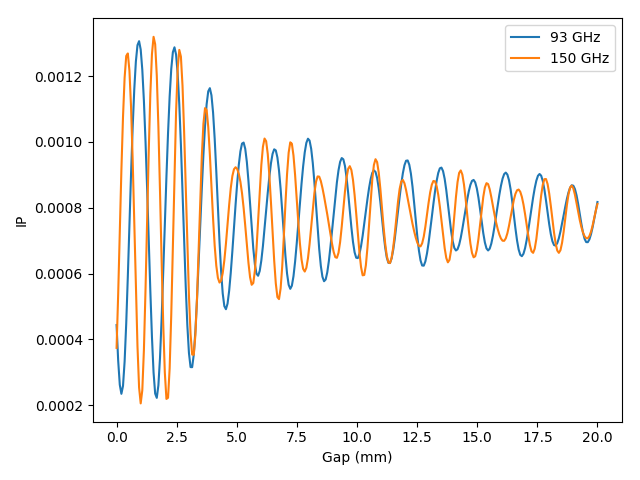
\includegraphics[width=.8\linewidth]{ip_vs_gap_filter_only.png}
  \caption{$IP$ coefficient as a function of distance for a system with just two aluminum filters separated by a gap.
  The incident angle is 7.5$\degree$, and frequencies of both 93 and 150 GHz are shown.
  }
  \label{fig:IP_vs_distance}
\end{figure}



\begin{table}[h]
\centering

\begin{tabular}{|c|c|c|c|c|}
\hline
$\theta $       & \multicolumn{2}{|c|}{Aluminum Filter IP} & \multicolumn{2}{|c|}{Aluminum Filter IP}           \\
\hline
 & 95 GHz & 150 GHz & 95 GHz & 150 GHz\\
 \hline
$7.5   \degree$& $6.69 \times 10^{-4}$ & $2.86 \times 10^{-5}$ & $3.88 \times 10^{-4}$ & $3.86 \times 10^{-4}$ \\
$10.0  \degree$& $1.20 \times 10^{-3}$ & $5.14 \times 10^{-5}$ & $6.79 \times 10^{-4}$ & $7.03 \times 10^{-4}$ \\
$12.5  \degree$& $1.90 \times 10^{-3}$ & $8.10 \times 10^{-5}$ & $1.04 \times 10^{-3}$ & $1.13 \times 10^{-3}$ \\
$15.0  \degree$& $2.79 \times 10^{-3}$ & $1.17 \times 10^{-4}$ & $1.47 \times 10^{-3}$ & $1.72 \times 10^{-3}$ \\
\hline
\end{tabular}
\caption{ Above are the band averaged IP coefficients for the window and aluminum filters at 93 and 150 GHz. $\theta$ is the incident angle of the light
on the surface.
}
\label{table:IP_coeffs}
\end{table}



\section{Optical Chain}
The optical chain used for the small aperture is given in table \ref{table:small_aperture_optical_chain}.



\begin{table}
\centering
\begin{tabular}{|c|c|c|c|}
\hline
Name & Temp & Abs [93 GHz, 150 GHz] & Refl \\
\hline
Window		& 300.0  & [0.005,0.010]	&0.010 \\
IRShader1	& 298.0  & [0.001,0.001]	&0.000 \\
IRShader2	& 293.0  & [0.001,0.001]	&0.000 \\
IRShader3	& 290.0  & [0.001,0.001]	&0.000 \\
IRShader4	& 276.0  & [0.001,0.001]	&0.000 \\
AluminaF	& 82.00  &  NA			   	&0.020 \\
IRShader1	& 76.00  & [0.001,0.001]	&0.000 \\
IRShader2	& 70.00  & [0.001,0.001]	&0.000 \\
IRShader3	& 65.00  & [0.001,0.001]	&0.000 \\
IRShader4	& 61.00  & [0.001,0.001]	&0.000 \\
AluminaF	& 42.00  &  NA			   	&0.020 \\
\hline
\multicolumn{4}{|c|}{HWP} \\
\hline
AluminaF	& 40.00  &  NA			   	&0.020 \\
AluminaF	& 5.000  &  NA			   	&0.020 \\
LowPass1	& 4.000  & [0.010,0.010]	&0.050 \\
Aperture	& 1.000  & NA	       		&NA	   \\
Lens		& 1.000  &  NA			   	&0.006 \\
Lens		& 1.000  &  NA			   	&0.006 \\
LowPass1	& 0.100  & [0.010,0.010]	&0.050 \\

\hline
\end{tabular}
\caption{ Above are the band averaged IP coefficients for the window and aluminum filters at 93 and 150 GHz. $\theta$ is the incident angle of the light
on the surface.
}
\label{table:small_aperture_optical_chain}
\end{table}



\section{Results}
$\A4$ for a detector at the edge of the array for various FOV's are given in Table \ref{table:HWPSS}.
I am only giving results in $K_\text{CMB}$ because the HWPSS in pW is proportional to the efficiency of the aperture,
which depends on the F-Number.
Because you can have different F-numbers for the same FOV, this would add another dimension to the input.
The aperture efficiency cancels out when converting to $K_\text{CMB}$, so we only get one value for each FOV.
I can include different F-Numbers in the future if people are interested.

\begin{table}[h]
\centering

\begin{tabular}{|c|c|c|}
\hline
$\theta$ & \multicolumn{2}{|c|}{$\A4 $ (mK$_\text{CMB}$)} \\
\hline
      & Aluminum Filter IP   & Window IP            \\
\hline
15$\degree$  & 4.52  & 5.88 \\
20$\degree$  & 13.9 & 18.1  \\
25$\degree$  & 43.6 & 57.1   \\
30$\degree$  & 95 & 124.1 \\\hline
\end{tabular}
\caption{ $\A4$ for various incident angles
}
\label{table:HWPSS}
\end{table}

\end{document}

